%%%%%%%%%%%%%%%%%%%%%%%%%%%%%%%%%%%%%%%%%%%%%%%%%%%%%%%%%%%%%%%%%%%%%%%%%
%%%%%%%%						Preamble						  %%%%%%%
%%%%%%%%%%%%%%%%%%%%%%%%%%%%%%%%%%%%%%%%%%%%%%%%%%%%%%%%%%%%%%%%%%%%%%%%%
\RequirePackage[l2tabu, orthodox]{nag} % tells you of any bad LaTeX usage

% choose parameter accordingly: twoside for Viva Docs, oneside for final submission
\documentclass[oneside]{um}

%%%%%%%%%%%%%%%%%%%%%%%%%%%%%%%%%%%%%%%%%%%%%%%%%%%%%%%%%%%%%%%%%%%%%%%%%
%%%%%%%%						Packages						  %%%%%%%
%%%%%%%%%%%%%%%%%%%%%%%%%%%%%%%%%%%%%%%%%%%%%%%%%%%%%%%%%%%%%%%%%%%%%%%%%
%\listfiles %used packages will be isted at the bottom of the .log file

%%%%%%%%%%%%%%%%%%%%%%%%%%%%%%%%%%%%%%%%%%%%%%%%%%%%%%%%%%%%%%%%%%%%%%%%%
%%%%%%%%						Data							  %%%%%%%
%%%%%%%%%%%%%%%%%%%%%%%%%%%%%%%%%%%%%%%%%%%%%%%%%%%%%%%%%%%%%%%%%%%%%%%%%
\title{Anomaly Detection Using\\Machine Learning\\Techniques for Beam\\Injections from the SPS\\ to the LHC at CERN}
\tagline{}
\author{Marc Ferriggi}
\supervisor{Dr. Gianluca Valentino}
\department{Department of Computer Science}
\faculty{Faculty of ICT}
\degree{B.Sc. (Hons.) Computing Science AND Statistics and Operations Research}
\doctype{FYP}
\degreedate{May, 2019}

%%%%%%%%%%%%%%%%%%%%%%%%%%%%%%%%%%%%%%%%%%%%%%%%%%%%%%%%%%%%%%%%%%%%%%%%%
%%%%%%%%					Document Settings					  %%%%%%%
%%%%%%%%%%%%%%%%%%%%%%%%%%%%%%%%%%%%%%%%%%%%%%%%%%%%%%%%%%%%%%%%%%%%%%%%%
\graphicspath{{./images/}}
\makeindex

%%%%%%%%%%%%%%%%%%%%%%%%%%%%%%%%%%%%%%%%%%%%%%%%%%%%%%%%%%%%%%%%%%%%%%%%%
\begin{document}
	\frontmatter 
	\maketitle
	\begin{originality}
\end{originality}    
	%\begin{dedication}
%\end{dedication}

        % include a dedication.tex file
	\begin{acknowledgements}
I'd like to first and foremost thank my supervisor Dr. Gianluca Valentino, this work wouldn't have been possible without his constant patience and support. I'd also like to thank my parents and family who have always believed in me and supported me financially to help me achieve my goals.
\end{acknowledgements}   % include an acknowledgements.tex file
	%% For tips on how to write a great abstract, have a look at
%%	-	https://www.cdc.gov/stdconference/2018/How-to-Write-an-Abstract_v4.pdf (presentation, start here)
%%	-	https://users.ece.cmu.edu/~koopman/essays/abstract.html
%%	-	https://search.proquest.com/docview/1417403858
%%  - 	https://www.sciencedirect.com/science/article/pii/S037837821830402X

\begin{abstract}

\end{abstract}\if@openright\cleardoublepage\else\clearpage\fi
	\tableofcontents*\if@openright\cleardoublepage\else\clearpage\fi
	\listoffigures*\if@openright\cleardoublepage\else\clearpage\fi
	\listoftables*\if@openright\cleardoublepage\else\clearpage\fi
	%% will only print what is used ... useful.
%% also acronyms are clickable, which is awesome

%%To reference, first time: \ac 
%%Other times \acs

\chapter*{List of Abbreviations}
               
\begin{acronym}\itemsep-20pt\parsep-20pt %% if you remove these spacing params this list becomes huge!
	\acro{BCT}{Beam Current Transformers}
	\acro{BLM}{Beam Loss Monitors}
	\acro{BPM}{Beam Position Monitors}
	\acro{BQM}{Beam Quality Monitor}
	\acro{CERN}{European Organization for Nuclear Research}
	\acro{Gy/s}{Grays per Second}
	\acro{IQC}{Injection Quality Check}
	\acro{LHC}{Large Hadron Collider}
	\acro{LS}{Logging Service}
	\acro{MJ}{Mega Joule}
	\acro{MKI}{LHC injection kicker systerm}
	\acro{mm}{millimetres}
	\acro{PCA}{Principal Component Analysis}
	\acro{RF}{Radiofrequency}
	\acro{SIS}{Software Interlock System}
	\acro{SPS}{Super Proton Synchrotron}
	\acro{TCDI}{Transfer Line Collimator}
	\acro{TDI}{Beam Absorber for Injection}
	\acro{TL}{Transfer Line}
%    \acro{BUT}{Block Under Test}%
%    \acrodefplural{BUT}{Blocks Under Test}%    
\end{acronym}
\if@openright\cleardoublepage\else\clearpage\fi
	
	%% Note: always use \input as you cannot nest \includes (amongst other things)
	\pagestyle{umpage}
	\mainmatter 
	\chapter{Introduction}

%\section{The LHC Machine}
%Establishing a territory:
\paragraph{ }The \ac{LHC} is a two-ring-superconducting-hadron accelerator and collider installed at the \ac{CERN} between the years 1984 and 1989 \cite{Evans2008}. The collider is 26.7km long and its purpose is to accelerate and collide two heavy ion beams \cite{Valentino2017}.

\paragraph{ }In order to operate the \acs{LHC} with a centre-of-mass energy of 14 \ac{TeV}, twelve injections from the \ac{SPS} consisting of a number of proton bunches of around 1 \ac{MJ} of stored energy are required \cite{Drosdal2011}. Thus, in order to fill the \acs{LHC}, approximately 4 minutes per beam is required. Furthermore, the whole experiment process of filling the LHC, performing the required checks, running the tests and dumping the beam should take a theoretical minimum of 70 minutes \cite{Evans2008}. However, from past experiences, this is expected to take longer, partly due to unsuccessful or anomalous proton injections to the \acs{LHC}. 

\paragraph{ }Clearly, filling the \acs{LHC} is a challenging task given the high energy of the beam, the very small apertures and the delivery precision's tight tolerances. The beam must pass through many accelerators and transfer lines before reaching the \acs{LHC}. During this process the beam must be monitored, thus multiple sensors are installed around the \acs{CERN} particle accelerator complex \cite{Lefevre2008} which gather readings and data that can be used to check the quality of the injected beam. 

%%Establishing a Niche:
\paragraph{ }  For this particular study, data generated from the sensors around the injection from the \acs{SPS} to the \acs{LHC} will be of particular interest (Figure \ref{fig::SPStoLHCInjection}). As the first beam (Beam 1) leaves the \acs{SPS}, it must pass through the transfer line TI2, while the second beam (Beam 2) must pass through TI8. The data from sensors around these transfer lines as well as at some points around the \acs{LHC} and \acs{SPS} will be used in this study and are stored using \acs{CERN}'s \ac{LS} \cite{Roderick2013}. While many studies have been made using this logged data and lots of statistical tests have been done with regards to injection quality checks for the \acs{LHC} (such as \cite{Drosdal2011} and \cite{Kain2010}), no literature was uncovered where researchers used unsupervised machine learning methods to analyse this particular data.

\begin{figure}[t]
	\centering
	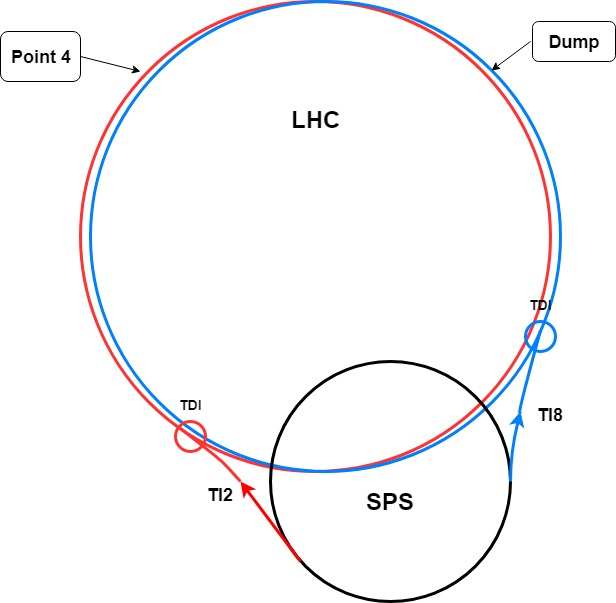
\includegraphics[width=0.6\textwidth]{CERNComplex}
	\caption[The CERN Particle Accelerator Complex]{Diagram of the particular area of interest of the CERN Particle Accelerator Complex for this study}
	\label{fig::SPStoLHCInjection}
\end{figure}

%% On the Current IQC software and cause of anomalies
\paragraph{ }Furthermore, the \ac{IQC} software currently installed has a set of hard-coded rules for detecting anomalies in the \acs{SPS}-\acs{LHC} injection \cite{Drosdal2011}, however there are documented cases in the past where situations occurred which were outside the originally foreseen rules and were therefore not caught as anomalies. Apart from causing experiments to fail, these anomalous injections could be very costly as a lot of data must be examined after such failures which wastes time that could be used to run more experiments \cite{Halilovic2018}. 

\paragraph{ }The major cause of these anomalies is due to the fact that the machine is so large, and needs to be so precise, that minor ground motions over time affect the tilts in the quadrupole magnets which thus affect the orbit of the beam. Figure \ref{fig::AnomalousInjections} highlights two possible cases of anomalous injections. The first case shows what happens to the beam when the \acs{BPM} gives a high \ac{MSE} reading with respect to its original position in the first injection of the season. The second case shows what happens to the beam when there is a high loss recorded by the \acs{TDI} \acs{BLM}.

\begin{figure}[t]
	\centering
	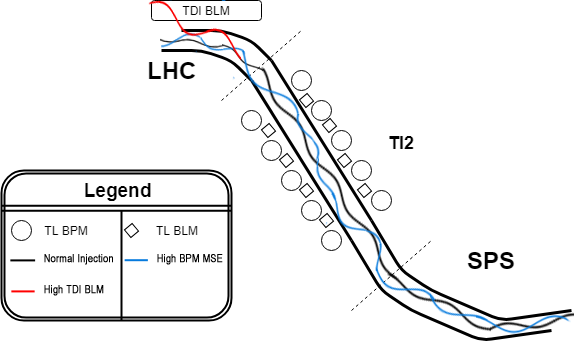
\includegraphics[width=0.6\textwidth]{AnomalousInjections}
	\caption[Anomalous Injections]{Examples of Anomalous Beam Injections showing the locations of the BPMs and BLMs in the transfer line}
	\label{fig::AnomalousInjections}
\end{figure}

%Thesis Statement:
\paragraph{ }The purpose of this study is to apply unsupervised anomaly detection algorithms to try solve the problem of detecting anomalous injections with the hopes of finding a technique that will detect the anomalies not being picked up by the \acs{IQC}. This can help researchers understand the source of these anomalies and improve the \acs{LHC} machine availability and performance reach in terms of beam lifetime, beam stability and luminosity.

%%TO DO:
%SIGNPOSTING!!!!!
\paragraph{ }In Chapter 2, the background to the problem domain is explained in further detail with the intention of providing the reader with information needed to fully understand this study. Recent published material on anomaly detection in particle accelerators is also presented in this chapter. The methodology used to analyse the provided dataset can be found in Chapter 3 where work done on the entire data science process is presented. The results of this study are then presented in Chapter 4 and a detailed evaluation on the performance of the anomaly detection algorithms can be found in Chapter 5. Some final conclusions and suggestions for further work are then presented in Chapter 6. 
	\chapter{Background and Literature Review}


\section{Beam Instrumentation}
\label{sec::beam_instrumentation}
%Intro
\paragraph{ }Throughout this study, data recorded as the beam leaves the \acs{SPS} and enters the \acs{LHC} will be used as input parameters to the chosen anomaly detection algorithms. This data was recorded using different censors located in different parts of the injection life cycle. This section describes the different types of censors that were used to collect the data, highlighting the particular details which need to be considered when analysing this data.

%BLMs & TDI BLMs
\paragraph{ }The \ac{BLM} are some of the most safety critical modules of the \acs{LHC} because a loss of a very small fraction of this beam may damage parts of the machine or cause a quench in the superconducting magnets \cite{Holzer2006}. A high beam loss reading could also indicate over-injection. In fact, an injection of a high intensity beam into the LHC is only allowed if there is a low intensity bunch circulating the LHC in order to avoid settings errors \cite{Kain2010}. The \acs{BLM} module is the mostly used module in the current IQC software checks \cite{Drosdal2011}. The \acs{BLM}s must be reliable; the probability of not detecting a dangerous loss was found to be $5\times10^{-6}$ per channel and they are only expected to generate 20 false dumps per year \cite{Holzer2006}. The \acs{BLM}s are extensively logged to a database for offline analysis \cite{Holzer2006}. 

\paragraph{ }For this particular study, the readings logged for the \ac{TDI} \acs{BLM}s and the \ac{TL} \acs{BLM}s in TI2 and TI8 will be used (refer to Figure \ref{fig::SPStoLHCInjection}). These readings come in 10 second windows around the injection of a bunch in \ac{Gy/s}.

%BPMs
\paragraph{ }The \ac{BPM} were installed as a system for fast monitoring of the beam's position with respect to it's orbit drift \cite{Schmidt2006}. The trajectory offsets recorded by the \acs{BLM}s in the transfer lines must be minimised in order to reduce losses \cite{Drosdal2011}. In fact, if the change in orbit substantially exceeds its provided boundary values then the beam should be dumped \cite{Schmidt2006} so as to not cause any damage to the equipment. Unlike the \acs{TDI} \acs{BLM}s, the \acs{BPM} system is independent to the collimator system. For this study, the readings from the transfer line \acs{BPM}s around TI2 and TI8 will be used (refer to Figure \ref{fig::SPStoLHCInjection}). Raw values for these readings are stored by the \acs{LS} in \ac{mm} and are logged every 1 - 5 seconds on average.

%Abort Gap
\paragraph{ }When filling the \acs{LHC}, it is necessary to keep an abort gap of at least 3$\mu s$ in order to accommodate for the \ac{MKD} rise time \cite{Meddahi2010}. As the \ac{LHC} is filling to nominal intensity, this gap will be populated with un-trapped particles and particles leaking out of their \ac{RF} buckets \cite{Meddahi2010}. The \ac{AGM} was hence specifically designed to measure this particle population in the abort gap \cite{Lefevre2010}. This monitor can be found in Point 4 (refer to Figure \ref{fig::SPStoLHCInjection}) in the LHC \cite{Lefevre2010}. The raw values extracted for this study are stored in number of particles and come in 10 second groups around the moment of injection.
 
%SPS and LHC Intensities
\paragraph{ }The actual intensities of the circulating beam are measured by \ac{BCT}. For the \acs{LHC} in particular, a fast \acs{BCT} is used which is capable of monitoring a broad range of currents as it must be able to detect a single pilot bunch circulating the machine (of 10 $\mu$A) as well as the full nominal machine (over 0.5 mA) \cite{Jones2007}. These readings are then converted from amps to number of protons per beam and stored for analysis. The intensities for the \acs{LHC} come in 10 second groups around the moment of injection while the intensities for the \acs{SPS} give a single value of the intensity at the time of injection. 

%Number of Bunches
%TO DO


\section{Feature Scaling and Reduction Techniques}

%% Intro:
%% Curse of Dimensionality & Importance of Normalisation
\paragraph{ }Feature Scaling and Feature Reduction are two important pre-processing steps that should be considered when using machine learning in the data science process. Standard Scaling in particular will be used in this study as a pre-processing step to \ac{PCA}. Standard Scaling ensures that all the features have the properties of a standard normal distribution \cite{Scikitlearn}, which is especially important since \acs{PCA} involves finding the components that maximise the variance \cite{Shlens2014}. 

\paragraph{ }Apart from scaling, another challenge for outlier detection algorithms is data involving high dimensions since the contrast between different points diminishes as the number of dimensions increases \cite{Zimek2012}. This phenomenon is known as `The Curse of Dimensionality' and a technique to reduce the effect of this phenomenon is to use a dimension reduction technique and run the outlier detection algorithm on this new lower-dimensioned dataset. In this study, \acs{PCA} will be used as a dimension reduction technique.

%% PCA:
\paragraph{ }\acs{PCA} uses statistical and mathematical techniques to reduce the dimension of large data sets, thus allowing a large data set to be interpreted in less variables called principal components \cite{Richardson2009}. This technique works with the hope that the variance explained by an acceptably small number of principal components is large enough to explain the underlying structure of the dataset reasonably \cite{Shlens2014}. In fact, this non-parametric method has been used as a means of revealing the simplified structures' underlying complex datasets with minimal effort. The fact that this technique is non-parametric gives it the advantage that each result is unique and only dependent on the provided data set since no parameter tweaking is required \cite{Shlens2014}, however this is also a weakness of \acs{PCA} as there is no way of exploiting prior expert knowledge on the data set.

\section{Unsupervised Anomaly Detection Techniques}

\paragraph{ }Unsupervised machine learning algorithms refer to the class of machine learning algorithms where only the input features are available to the learner as there is no access to output labels corresponding to each input feature vector, or the aim of the algorithm is simply to observe or detect patterns in the available data. A. Hyv\"{a}rinen states in \cite{Hyvarinen2015} that some of the goals of unsupervised learning include data visualisation, noise reduction, feature extraction and finding interesting components; all of which are of particular interest in this study.

\paragraph{ }\ac{DBSCAN} and \ac{LOF} will both be used as unsupervised anomaly detection algorithms to detect and classify anomalous injections of the past year. Furthermore when working in 3 dimensions or less, these points can also be visualised to help the reader understand better the cause of these anomalies. 

\paragraph{ }\acs{DBSCAN} was created out of the necessity of having a clustering algorithm with the following requirements:
\begin{enumerate}
	\item ``Minimal requirements of domain knowledge to determine the input parameters,''
	\item ``Discovery of clusters with arbitrary shape,'' and
	\item ``Good efficiency on large databases'' \cite{Ester1996}
\end{enumerate}
\acs{DBSCAN} manages to attain these requirements by viewing clusters as ``areas of high density separated by areas of low density'' \cite{Sklearn2}. The points with a lower density will thus be considered as anomalies when compared to the regular clusters which have a higher density. This algorithm also introduces the concept of \textit{core samples} which was then used in the design of other unsupervised anomaly detection algorithms such as \acs{LOF}. 

\paragraph{ }The word \textit{factor} in \acs{LOF} refers to a ``degree of outlier-ness'' that this algorithm considers for each point in the data rather than using the concept that ``being an outlier is binary'' \cite{Breunig2000}. This algorithm uses a clustering technique which takes concepts from \acs{DBSCAN} to measure the \acs{LOF} of each point where a \acs{LOF} value greater than 1 implies that the point has a lower density than its neighbours and is thus probably an outlier.
%%To DO: MORE ON LOF

\section{Anomaly Detection at CERN}

\paragraph{ }In the paper released entitled ``Opportunities in Machine Learning for Particle Accelerators'' \cite{Edelen2018}, it was stated that due to the ''large number of process variables, non-linear behaviour, and many interacting subsystems,'' conventional analysis techniques on today's particle accelerator data is often insufficient and thus machine learning could be used as a means of anomaly detection. Furthermore, the authors also stated that these techniques could be used to detect ``subtle behaviours of key variables prior to negative events'' and they can also be used to ``identify and throw away bad signals.''

\paragraph{ }In his Master's Thesis, A. Halilovic used anomaly detection techniques solely on data obtained from the injection kicker magnets \cite{Halilovic2018}. Halilovic made use of a \ac{GMM} and Isolation Forests to detect anomalies however found that the best performance achieved by his proposed pipeline ``leaves something to be desired'' as too many anomalies were not correctly classified. The author also goes on to suggest that analysing \acs{LHC} data using the \acs{LOF} class provided in `\textit{scikit-learn}' could lead to interesting results.

\paragraph{ }Wielgosz, \textit{et. al.} also wrote a scientific paper on using anomaly detection techniques on the \acs{LHC} magnets \cite{Wielgosz2017}. This time, the authors went for a supervised approach and used Recurrent Neural Networks. They found that using adaptive quantisation to reduce 20-bit inputs into a 4-bit representation was an essential step in improving the algorithm's performance. The authors also stated that these anomaly detection techniques being proposed should not only be considered useful for \acs{CERN} equipment but also useful in the broader field of anomaly detection on time series data.

\paragraph{ }In 2017, Valentino \textit{et. al.} released a paper on using anomaly detection techniques ``to detect minor changes in the loss maps over time due to collimator settings errors or orbit variations'' \cite{Valentino2017}. The authors used \acs{PCA} as a dimension reduction technique and then applied \acs{LOF} on the resulting 2 dimensional data. Their proposed method was shown to positively identify these anomalous loss maps based solely on \acs{BPM} and \acs{BLM} readings. Furthermore, they proposed using this technique to monitor losses during fills of the \acs{LHC}.

\section{Software Implementation}
\paragraph{ }Although performance of k-means and k-Nearest Neighbours is not as optimal as in other Python packages such as `\textit{PyMVPA}' \cite{PyMVPA} or `\textit{shogun}' \cite{Shogun} (see Table 1 in \cite{Pedregosa2011}), it was decided to use the `\textit{scikit-learn}' machine learning package for this study due to its ``state-of-the-art implementation'' and ``easy-to-use interface tightly integrated with the Python language'' \cite{Pedregosa2011}. Furthermore, the algorithms implemented using this package can be ``used as building blocks for approaches specific to a use case'' \cite{Pedregosa2011} which will be useful if one would like to extend the scope of this study.
%	\input{chap3/materials_and_methods_main}
%	\input{chap4/results_and_discussion_main}
%	\input{chap5/evaluation_main}
%	\input{chap6/conclusions_main}
%	\appendix
%	\input{appA/appendix_a_main}     % these are just test names as I didn't know what you'd want
%	\input{appB/appendix_b_main}    
%	\input{appC/appendix_c_main} 
	
	{\backmatter
		% Bibliography
		\if@openright\cleardoublepage\else\clearpage\fi
		%\bibliographystyle{um-plainnat} %% specific plainnat does not show url for articles
		\bibliographystyle{IEEEtran}
		{\footnotesize\bibliography{Chapter2/background_biblio}}
		\printindex
	}
	
	
\end{document}